\begin{section}{Results}
  \label{sec:results}
  We now present the results of a simulation of (**) neutrinos 
with mass 0.2eV and (**) dark matter particles. The simulation 
is done in a box of size $500 Mpc/h$. As noted above, initial 
conditions for dark matter particles are produced at $z=100$ 
whereas neutrinos are introduced at $z=10$. We take cosmological 
parameters which are in line with the most recent Planck results 
\cite{bib:Planck2015}: $h=0.67,\, \Omega_b=0.05, \Omega_c=0.27, 
\sigma_8=??,\, n_s=0.67 $, and

\begin{equation}
  \Omega_\nu = \frac{m_\nu}{93.14 h^2}
\end{equation}
We assume a flat universe and so set $\Omega_\Lambda=1-\Omega_m=1-\Omega_b-\Omega_c-\Omega_\nu$.

\par The density power spectra of the four velocity bins are depicted in Fig. \ref{fig:denpowerfig}.
Neutrinos with smaller initial velocities have greater power at all scales 
with the difference between the velocity bins increasing at smaller scales. 
This is to be expected as less energetic neutrinos are more easily trapped 
in potential wells and thus tend to cluster. This also results in the power 
spectra of the neutrinos with the smallest initial velocities deviating the 
most from linear theory. The velocity power spectra are shown in Fig. \ref{fig:velpowerfig}.
A similar pattern is evident as neutrinos with smaller initial velocity have
greater power at all scales. The velocities of less energetic neutrinos are
more likely to be correlated (particularly over small scales) as they will
more easily be focused into clusters with a coherent velocity than neutrinos
with large initial velocities. 

\par Lastly, the dipole correlation functions for each velocity bin are 
shown in Fig. \ref{fig:dipolefig}. Despite small deviations, the dipole
does not seem to differ significantly between the velocity bins. 

\begin{figure}[htbp]
  \begin{center}
    \includegraphics[width=0.5\textwidth]{./figures/DensityPowerSpectra/denpower.pdf}
    \caption{(Placeholder) Density power spectra of the four neutrino velocity bins
	      at z=0 (solid lines). Also plotted are the power spectra predicted by
	      linear theory (dashed lines).}
    \label{fig:denpowerfig}
  \end{center}
\end{figure}

\begin{figure}[htbp]
  \begin{center}
    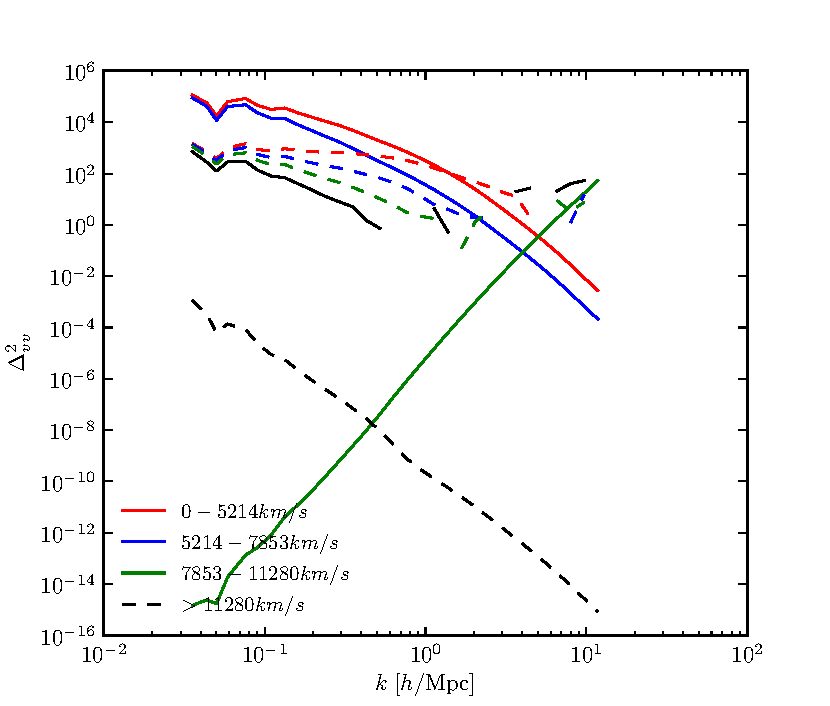
\includegraphics[width=0.5\textwidth]{./figures/VelPowerSpectra/velpower.pdf}
    \caption{(Placeholder) Velocity power spectra of the four neutrino velocity
	      bins at z=0 (dashed lines) compared with the reconstructed velocity
	      power spectra (solid lines).}
    \label{fig:velpowerfig}
  \end{center}
\end{figure}


\begin{figure}[htbp]
  \begin{center}
    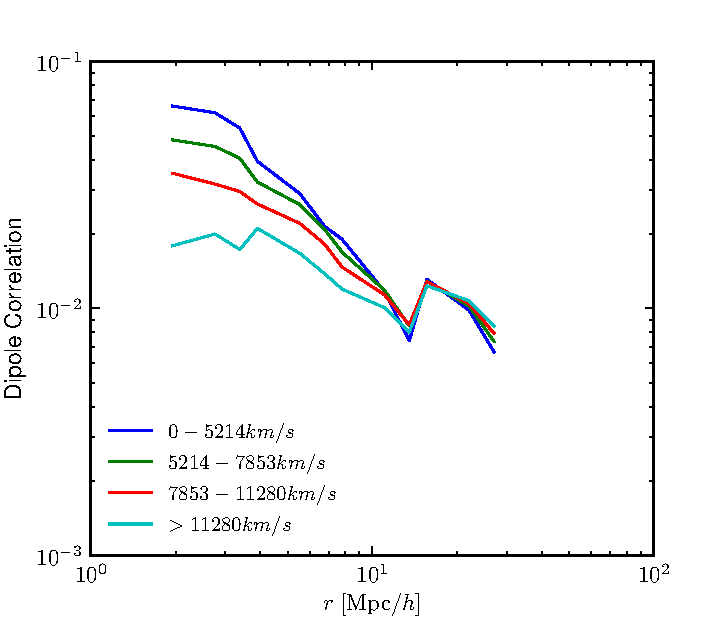
\includegraphics[width=0.5\textwidth]{./figures/Dipole/dipolefig.pdf}
    \caption{(Placeholder) Dipole correlation functions for each neutrino
	      velocity bin at z=0.}
    \label{fig:dipolefig}
  \end{center}
\end{figure}


\end{section}
